\documentclass[conference]{IEEEtran}
% Research draft. Preliminary results and implementation details require
% reconciliation with the approved checkpoints and evaluator before submission.
\usepackage{cite}
\usepackage{amsmath,amssymb,amsfonts}
\usepackage{graphicx}
\usepackage{booktabs}
\usepackage{array}
\usepackage{url}
\usepackage{tikz}
\usetikzlibrary{arrows.meta,positioning,fit,calc}
% Figure-only palette; IEEEtran typography and page layout are unchanged.
\definecolor{diagramNavy}{RGB}{32,58,82}
\definecolor{diagramTeal}{RGB}{24,115,128}
\definecolor{diagramSoft}{RGB}{238,243,247}

\begin{document}
\title{Learning Collaborative Action Policies for Humans and Robots with Intent Awareness}
\author{\IEEEauthorblockN{Dao Duy Hung}
\IEEEauthorblockA{Affiliation and email to be confirmed}}
\maketitle

\begin{abstract}
Human--robot collaboration requires a robot to coordinate the timing and location of its actions with a human partner whose future behavior is not fully observable. A policy that waits until every human event is completed may introduce avoidable delays; a policy that commits prematurely to an inaccurate prediction may instead create rework or unsafe interaction. This work studies how a unified robot action policy can learn to exploit short-horizon human-motion forecasts while retaining the ability to correct decisions based on updated observations. Action Chunking with Transformers (ACT) provides the imitation-learning backbone and ManiCast serves as a replaceable source of predicted human motion. We formulate three complementary learning questions: useful early action, selective dependence on forecasts, and correction after prediction errors or human goal changes. The evaluation design separates task success from anticipation, waiting time, physical validity, and forecast sensitivity. Preliminary project evaluations reveal task-specific strengths and failures but do not yet provide a statistically verified improvement in collaboration efficiency or robustness. Accordingly, this paper presents a research formulation, candidate learning mechanisms, controlled comparisons, and the evidence required to validate them.
\end{abstract}
\begin{IEEEkeywords}
human--robot collaboration, imitation learning, anticipatory action, human-motion forecasting, action chunking, intent awareness
\end{IEEEkeywords}

\section{Introduction}
Effective human--robot collaboration (HRC) involves more than the accurate execution of individual manipulations. The actions of the two partners may depend on one another in space and time. When the robot begins a task-dependent movement only after a decisive human event has become observable, part of the work that could have overlapped is delayed. However, acting toward a guessed goal before the human's choice is sufficiently clear can create unnecessary travel, inappropriate contact, or a failed task. The robot must therefore learn not only \emph{what} to do but also \emph{when} and \emph{where} an action is useful.

Joint-action theory motivates coordination through shared task representations and anticipation of the partner's behavior \cite{sebanz2006}. Measures of human--robot team fluency further distinguish successful manipulation from smooth, timely collaboration \cite{hoffman2007,hoffman2019}. Motion forecasting provides a possible source of advance information. ManiCast studies cost-aware forecasting of human motion for collaborative manipulation and emphasizes the effect of prediction errors on downstream decisions \cite{kedia2023}. In parallel, Action Chunking with Transformers (ACT) learns sequences of robot actions from demonstrations \cite{zhao2023}; Diffusion Co-Policy provides another example of learning coordinated behavior from interaction data \cite{ng2024}.

Connecting these capabilities directly does not guarantee that the learned policy will use future-motion information. A network may ignore the forecast input, act early without changing task duration, or continue an obsolete action chunk after the human changes course. These are policy-learning and execution problems, distinct from prediction accuracy alone. The central research question is how a unified policy can use predicted human behavior to initiate \emph{useful} action early while adapting to uncertainty and new observations.

The study addresses three questions. First, can forecast-conditioned learning improve the onset of useful robot activity and reduce unnecessary waiting? Second, can the policy respond to informative forecast changes without becoming unstable under unreliable predictions? Third, can it correct goal-dependent actions when the forecast is wrong or the human changes intention, while satisfying physical constraints? We treat ManiCast as one possible forecaster; the intended methodological contribution is not an intent classifier, a new prediction network, or task-specific hand-coded control laws.


\begin{figure}[t]
\centering
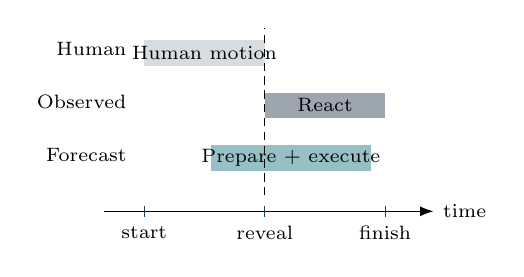
\begin{tikzpicture}[x=0.51cm,y=0.67cm, font=\scriptsize,>=Latex]
\draw[->] (0,0)--(8.2,0) node[right]{time};
\foreach \x/\s in {1/start,4/reveal,7/finish} {
  \draw[diagramNavy] (\x,-0.1)--(\x,0.10);
  \node[below] at (\x,-0.10) {\s};}
\node[anchor=east] at (0.8,3.07){Human};
\node[anchor=east] at (0.8,2.07){Observed};
\node[anchor=east] at (0.8,1.07){Forecast};
\fill[diagramNavy!18] (1,2.76) rectangle (4.0,3.25);
\node at (2.50,3.01){Human motion};
\fill[diagramNavy!45] (4,1.76) rectangle (7,2.25);
\node at (5.50,2.01){React};
\fill[diagramTeal!45] (2.65,0.76) rectangle (6.65,1.25);
\node at (4.65,1.01){Prepare + execute};
\draw[densely dashed] (4,0.3)--(4,3.47);
\end{tikzpicture}
\caption{Illustrative action timing. Forecast access can enable preparation before the human event becomes observable. Earlier motion is not itself evidence of reduced waiting or task completion time.}
\label{fig:timing}
\end{figure}

\section{Related Work}
\subsection{Anticipation and coordination}
Sebanz et al. characterize joint action as coordinated behavior among multiple agents \cite{sebanz2006}. Hoffman and Breazeal examine anticipatory decisions in human--robot teams \cite{hoffman2007}, and Hoffman reviews measures of teamwork fluency \cite{hoffman2019}. These studies motivate the distinction between early movement and useful anticipation. A meaningful timing measure must account for task dependencies, human waiting, and the consequence of an early commitment.

\subsection{Human-motion forecasting}
Forecasts represent possible future movement rather than observed future ground truth. ManiCast considers prediction errors according to their effect on collaborative planning \cite{kedia2023}. A motion trajectory can reveal both the direction of human movement and the evolving region of interaction, although its task meaning depends on the surrounding scene and activity. Thus, forecast quality alone does not specify the correct robot action. The present work uses forecasts as policy inputs, leaving the predictor replaceable.

\subsection{Learning and adapting robot actions}
Learning from demonstration supports robot manipulation when explicit procedural rules are cumbersome \cite{argall2009}. ACT produces continuous action chunks from observations \cite{zhao2023}. Diffusion Co-Policy addresses learned coordination in collaborative tasks \cite{ng2024}. One difficulty with behavior cloning is distribution shift: the learner may encounter states absent from expert demonstrations. DAgger addresses this issue by incorporating expert feedback on states visited by the current policy \cite{ross2011}. Human goal changes and incorrect commitments create analogous off-demonstration states that should be represented in corrective training data.

\section{Problem Definition}
\begin{figure*}[t]
\centering
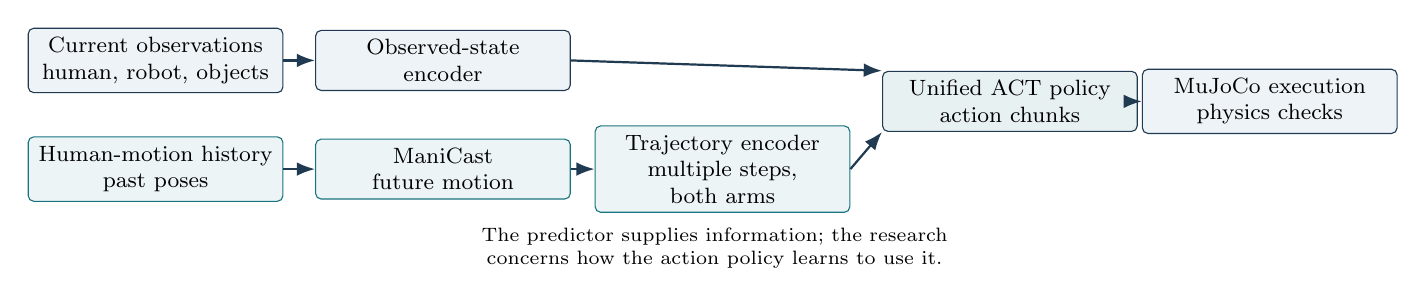
\begin{tikzpicture}[>=Latex, font=\footnotesize,
 n/.style={draw=diagramNavy, rounded corners=2pt, fill=diagramSoft,
           align=center, minimum height=0.73cm, text width=3.00cm},
 pred/.style={draw=diagramTeal, rounded corners=2pt, fill=diagramTeal!8,
           align=center, minimum height=0.73cm, text width=3.00cm},
 flow/.style={->, thick, draw=diagramNavy}]
\node[n] (ob) at (0,1.55) {Current observations\\human, robot, objects};
\node[pred] (hist) at (0,0.17) {Human-motion history\\past poses};
\node[n] (enc) at (3.65,1.55) {Observed-state\\encoder};
\node[pred] (mc) at (3.65,0.17) {ManiCast\\future motion};
\node[pred] (fenc) at (7.20,0.17) {Trajectory encoder\\multiple steps, both arms};
\node[n,fill=diagramTeal!10] (act) at (10.85,1.03) {Unified ACT policy\\action chunks};
\node[n] (phys) at (14.15,1.03) {MuJoCo execution\\physics checks};
\draw[flow] (ob)--(enc); \draw[flow] (hist)--(mc); \draw[flow] (mc)--(fenc);
\draw[flow] (enc.east)--(act.north west); \draw[flow] (fenc.east)--(act.south west);
\draw[flow] (act)--(phys);
\node[anchor=north,align=center,text width=10cm,font=\scriptsize] at (7.1,-0.46)
 {The predictor supplies information; the research concerns how the action policy learns to use it.};
\end{tikzpicture}
\caption{Conceptual forecast-conditioned policy. The diagram describes the intended information flow, not a verified final encoder or fusion implementation.}
\label{fig:framework}
\end{figure*}

Let $o_t$ denote observations available at time $t$, including the robot, human, objects, and task context. From human-motion history $h_{t-L:t}$, a forecaster $F$ produces a future trajectory
\begin{equation}
\hat{\mathcal H}_t=F(h_{t-L:t})=
\{\hat h_{t+\Delta},\ldots,\hat h_{t+K\Delta}\}.
\label{eq:forecast}
\end{equation}
The intended ManiCast interface retains multiple time steps over approximately one second, with upper-body joints from both arms. The exact deployed sampling and joint layout require code-level verification; reducing the forecast to only the terminal wrist position would discard trajectory-shape information that the research aims to test.

A shared policy $\pi_\theta$ generates an action chunk
\begin{equation}
\hat{\mathcal A}_t=\pi_\theta(o_t,\hat{\mathcal H}_t)=
\{\hat a_t,\ldots,\hat a_{t+H-1}\}.
\label{eq:policy}
\end{equation}
The task is represented through the observed scene and interaction rather than by a separate, manually assigned task-intent label. In this study, intent awareness is expressed by decisions about when a task-dependent action becomes useful and where the relevant human--robot interaction is likely to take place.

A causal deployment constraint is essential. At time $t$, the policy may use observations through $t$ and forecasts computed from them, but not ground-truth human poses from future time steps. Oracle future motion may be used only as a diagnostic control. We further distinguish reversible preparation from commitment to a specific goal. A successful policy may prepare early while deferring an irreversible movement until enough evidence is available.

\section{Proposed Learning Framework}
\subsection{Shared action-policy backbone}
The observation-only and forecast-aware configurations use the same robot action representation and physical task constraints. The candidate architecture encodes the observed scene and the forecast trajectory separately before combining their representations in ACT. This separation lets the learning system access current evidence even when a forecast is absent or contradicted. The exact fusion mechanism remains an implementation decision and must be reported from the trained code, not inferred from the conceptual diagram.

\subsection{Learning useful anticipation}
The training workflow begins with demonstrations from a physically constrained expert. Observation-based and forecast-aware demonstrations must use equivalent scenes, collision criteria, and success gates; otherwise, apparent forecast benefits may originate from differences in expert quality. A standard imitation objective is
\begin{equation}
\mathcal L_{\mathrm{BC}}=\mathbb E_{\mathcal D}
\left[\ell\bigl(\pi_\theta(o_t,\hat{\mathcal H}_t),
\mathcal A_t^*\bigr)\right].
\label{eq:bc}
\end{equation}
One proposed mechanism is to increase attention to onset and transition frames, where a small action error may have a larger effect on collaboration timing. A candidate weighted objective is
\begin{equation}
\mathcal L_{\mathrm{event}}=\mathbb E_{\mathcal D}
\left[\sum_{k=0}^{H-1} w_{t,k}
\ell(\hat a_{t+k},a^*_{t+k})\right].
\label{eq:event}
\end{equation}
Here $w_{t,k}$ is based on independently defined decision events. Equation~\eqref{eq:event} is a hypothesis to be tested, not an assertion about the final implemented objective. The effect of such weighting must be isolated with the same data, model capacity, and training budget. For latent-variable ACT models, KL regularization and latent-unit activity should also be monitored. Preventing latent collapse by itself does not prove that the policy uses forecasts.

\subsection{Selective forecast dependence}
A forecast can be wrong in destination, timing, or path. Such forecast faults differ from an actual human change of mind. Training and evaluation should therefore include nominal predictions, controlled faults, forecast masking, and newly observed motion contradicting an earlier prediction. The desired policy changes its action when the forecast is decision-relevant but avoids unnecessary motion when the forecast is irrelevant or unreliable.

To diagnose forecast dependence, we compare action outputs with the same observation $o_t$ but alternative forecasts $\hat{\mathcal H}_t$ and $\tilde{\mathcal H}_t$. This intervention reveals whether future-motion information changes the action. It does not establish that the change is beneficial; correctness and task outcome must be measured separately. Similarly, zero action difference is informative only when the substituted forecasts imply different useful actions.


\begin{figure}[t]
\centering
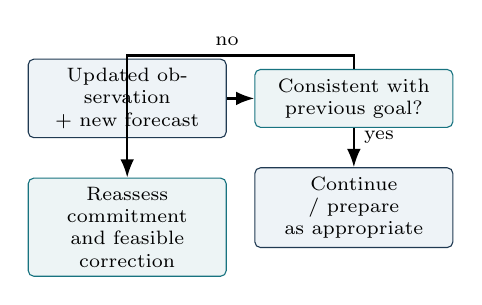
\begin{tikzpicture}[font=\scriptsize, >=Latex,
 node distance=0.27cm,
 b/.style={draw=diagramNavy,rounded corners=2pt,fill=diagramSoft,align=center,text width=2.28cm,minimum height=0.60cm},
 c/.style={draw=diagramTeal,rounded corners=2pt,fill=diagramTeal!8,align=center,text width=2.28cm,minimum height=0.60cm}]
\node[b] (a) {Updated observation\\+ new forecast};
\node[c,right=0.35cm of a] (b) {Consistent with\\previous goal?};
\node[b,below=0.50cm of b] (c) {Continue / prepare\\as appropriate};
\node[c,below=0.50cm of a] (d) {Reassess commitment\\and feasible correction};
\draw[->,thick] (a)--(b);
\draw[->,thick] (b)--node[right,near start]{yes} (c);
\draw[->,thick] (b.north) -- ++(0,0.17) -| node[above,pos=0.28]{no} (d.north);
\end{tikzpicture}
\caption{Decision-level interpretation of forecast updates. This is a learning target, not a separately implemented rule controller; feasible actions remain subject to physical constraints.}
\label{fig:update}
\end{figure}

\subsection{Correction after commitment}
The human may switch goals before or after the robot commits to a target-dependent movement. Before commitment, correction may require only a target update. After commitment, the robot may need to redirect, finish a safe intermediate motion, or acknowledge that a valid recovery is no longer feasible. We investigate corrective demonstrations collected from states reached by the current policy. The DAgger principle \cite{ross2011} offers one way to collect such examples before introducing reinforcement learning. Recovery should be evaluated by successful adaptation and physical validity, rather than assuming that recovery time should always be minimized.

\subsection{Execution and physical constraints}
Action chunks are executed with feedback from new observations. The chunk length, execution step, and forecasting cycle jointly limit responsiveness to human changes. Physical checks in MuJoCo include joint limits, collision and contact conditions, and human--robot clearance. These checks are distinct from learned behavior: a low imitation error or successful target placement does not guarantee physically valid execution.

\section{Experimental Design}
\subsection{Interaction patterns and scenarios}
The MuJoCo task suite covers three patterns: human-guided work, cooperative handling, and relatively independent concurrent work. It contains tasks designed to require correct spatial decisions, temporal alignment, or both. Cases include nominal interaction, forecast faults, and goal switches before or after commitment where meaningful. Task categories are inspired by the broader human--robot interaction literature and HRIBench \cite{hribench2026}, but all project scenes and metrics remain project-specific. Tasks whose experts or contact constraints have not passed feasibility checks must not enter a definitive comparison.

\subsection{Baselines}
\begin{table}[t]
\caption{Intended comparison conditions}
\label{tab:baselines}
\centering\footnotesize
\begin{tabular}{p{0.32\columnwidth}p{0.59\columnwidth}}
\toprule
Policy & Question tested\\
\midrule
Observed ACT & Performance using available observations without forecasts\\
History ACT & Added effect of past human motion alone\\
Direct forecast ACT & Effect of providing ManiCast predictions with ordinary imitation learning\\
Proposed variants & Added effect of each verified learning mechanism\\
\bottomrule
\end{tabular}
\end{table}
All configurations should be compared with matched human episodes, seeds, robot settings, and evaluator definitions. Development model names M0, M1-noH, and M* must be mapped to exact inputs, objectives, and checkpoints before publication; their names are not substitutes for architectural specifications.

\subsection{Evaluation criteria}
Task success is necessary but insufficient. We measure the first \emph{useful} robot action onset, human waiting, total task duration, task-specific synchronization, physical validity, forecast sensitivity, and recovery under controlled changes. An onset gain counts as a collaborative benefit only when it lowers waiting or completion time without unacceptable failures. Synchronization thresholds should reflect each task's dependency structure; project-defined TSync thresholds must not be presented as official HRIBench metrics.


\begin{table}[t]
\caption{Proposed task cases and key diagnostic questions}
\label{tab:scenario}
\centering\footnotesize
\begin{tabular}{p{0.30\columnwidth}p{0.57\columnwidth}}
\toprule
Case & Primary question \\
\midrule
Nominal & Is forecast-driven anticipation useful?\\
Forecast fault & Does the policy rely on wrong prediction?\\
Switch before commit & Can it defer or redirect a goal?\\
Switch after commit & Can it recover in a feasible state?\\
\bottomrule
\end{tabular}
\end{table}

\subsection{Ablations and error attribution}
The planned ablations remove forecast input, decision-event weighting, forecast-reliance mechanisms, or corrective data one at a time. Paired forecast swaps, masks, and contradictions test whether the policy actually uses predictions. Failure analysis is performed by task and execution phase to distinguish expert errors, dataset problems, observation errors, learned-action errors, evaluator mistakes, and physics violations. This audit should precede a decision to add more training or reinforcement learning.

\section{Preliminary Results and Evidence Boundaries}
\begin{figure}[t]
\centering
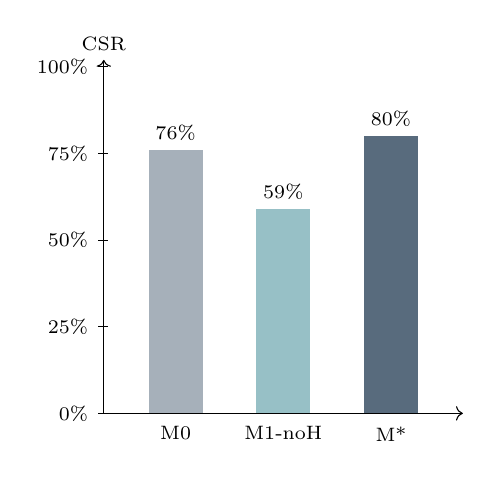
\begin{tikzpicture}[x=0.57cm,y=0.044cm,font=\scriptsize]
\draw[->] (0,0)--(0,102) node[above]{CSR};
\draw[->] (0,0)--(8,0);
\foreach \y in {0,25,50,75,100}{\draw (-0.12,\y)--(0.10,\y);\node[left] at (-0.13,\y){\y\%};}
\fill[diagramNavy!40] (1,0) rectangle (2.2,76);
\fill[diagramTeal!45] (3.4,0) rectangle (4.6,59);
\fill[diagramNavy!75] (5.8,0) rectangle (7,80);
\foreach \x/\v/\s in {1.6/76/M0,4/59/M1-noH,6.4/80/M*} {
\node[above] at (\x,\v){\v\%};\node[below] at (\x,-1){\s};}
\end{tikzpicture}
\caption{Development validation CSR reported on 19 Nov. 2026 (300 episodes, ten validation seeds). Descriptive, not a paired significance test or final benchmark.}
\label{fig:devcsr}
\end{figure}

An internal project validation dated 19 November 2026 describes 300 evaluation episodes over ten validation seeds and selected task/case conditions. The reported descriptive macro task-success rates are 0.76 for M0, 0.59 for M1-noH, and 0.80 for M*. These figures are development observations, not a verified overall model ranking. Confidence intervals are broad, paired statistical tests are absent, and the models behave differently across tasks. In particular, M* remained weak on I2 and on an I3 switch-after-commit case. Evaluator and metric definitions, including temporal synchronization and recovery-related measures, still require reconciliation.

A separate exploratory diagnostic investigated whether modifying latent regularization was sufficient to induce forecast usage. With the KL term disabled, 184 of 256 latent units were still inactive in the reported run. In a forecast-swap test, the median tool-center-point change was approximately 0.010 mm and direction correctness was 46\%. These measurements support investigating a specific conditioning failure mode. They do not demonstrate that every checkpoint ignores the forecast, nor do they establish the effect of any individual training mechanism.

Task completion and physical validity also differ in several evaluated cases. Violations of clearance or contact constraints cannot be removed from analysis simply because a goal was reached. Therefore, current evidence does not justify a final claim of earlier useful action, reduced total task time, statistically superior completion, or robust recovery. The next required steps are task-level audits, aligned evaluation metrics, paired rollouts, and verified corrective learning.

\section{Conclusion}
This work frames intent-aware human--robot collaboration as learning to act from uncertain future-motion information. The proposed ACT-based policy treats forecasts as decision-relevant but fallible inputs and separates preparation, commitment, and correction from the physical constraints of execution. The central test is whether the resulting policy can convert predicted human motion into timely, correctable, and physically valid robot behavior. Current development results identify meaningful research problems but remain preliminary. Controlled ablations and paired evaluations are required before the proposed mechanisms can be claimed as experimentally established contributions.

\begin{thebibliography}{00}
\bibitem{sebanz2006} N. Sebanz, H. Bekkering, and G. Knoblich, ``Joint action: Bodies and minds moving together,'' \emph{Trends in Cognitive Sciences}, 2006, doi: 10.1016/j.tics.2005.12.009.
\bibitem{hoffman2007} G. Hoffman and C. Breazeal, ``Effects of anticipatory action on human--robot teamwork efficiency, fluency, and perception of team,'' 2007, doi: 10.1145/1228716.1228718.
\bibitem{hoffman2019} G. Hoffman, ``Evaluating fluency in human--robot collaboration,'' \emph{IEEE Transactions on Human-Machine Systems}, 2019, doi: 10.1109/THMS.2019.2904558.
\bibitem{kedia2023} Kedia et al., ``ManiCast: Collaborative manipulation with cost-aware human forecasting,'' \emph{CoRL}, 2023. \url{https://proceedings.mlr.press/v229/kedia23a.html}.
\bibitem{zhao2023} T. Z. Zhao et al., ``Learning fine-grained bimanual manipulation with low-cost hardware,'' \emph{Robotics: Science and Systems}, 2023. \url{https://roboticsproceedings.org/rss19/p016.html}.
\bibitem{ng2024} E. Ng, Z. Liu, and M. Kennedy, ``Diffusion Co-Policy for synergistic human--robot collaborative tasks,'' \emph{IEEE Robotics and Automation Letters}, 2024. \url{https://arxiv.org/abs/2305.12171}.
\bibitem{argall2009} B. D. Argall et al., ``A survey of robot learning from demonstration,'' \emph{Robotics and Autonomous Systems}, 2009, doi: 10.1016/j.robot.2008.10.024.
\bibitem{ross2011} S. Ross, G. Gordon, and D. Bagnell, ``A reduction of imitation learning and structured prediction to no-regret online learning,'' \emph{AISTATS}, 2011. \url{https://proceedings.mlr.press/v15/ross11a.html}.
\bibitem{hribench2026} Liu et al., ``HRIBench,'' arXiv:2607.13056, 2026.
\end{thebibliography}
\end{document}